
%% bare_conf.tex
%% V1.3
%% 2007/01/11
%% by Michael Shell
%% See:
%% http://www.michaelshell.org/
%% for current contact information.
%%
%% This is a skeleton file demonstrating the use of IEEEtran.cls
%% (requires IEEEtran.cls version 1.7 or later) with an IEEE conference paper.
%%
%% Support sites:
%% http://www.michaelshell.org/tex/ieeetran/
%% http://www.ctan.org/tex-archive/macros/latex/contrib/IEEEtran/
%% and
%% http://www.ieee.org/

%%*************************************************************************
%% Legal Notice:
%% This code is offered as-is without any warranty either expressed or
%% implied; without even the implied warranty of MERCHANTABILITY or
%% FITNESS FOR A PARTICULAR PURPOSE! 
%% User assumes all risk.
%% In no event shall IEEE or any contributor to this code be liable for
%% any damages or losses, including, but not limited to, incidental,
%% consequential, or any other damages, resulting from the use or misuse
%% of any information contained here.
%%
%% All comments are the opinions of their respective authors and are not
%% necessarily endorsed by the IEEE.
%%
%% This work is distributed under the LaTeX Project Public License (LPPL)
%% ( http://www.latex-project.org/ ) version 1.3, and may be freely used,
%% distributed and modified. A copy of the LPPL, version 1.3, is included
%% in the base LaTeX documentation of all distributions of LaTeX released
%% 2003/12/01 or later.
%% Retain all contribution notices and credits.
%% ** Modified files should be clearly indicated as such, including  **
%% ** renaming them and changing author support contact information. **
%%
%% File list of work: IEEEtran.cls, IEEEtran_HOWTO.pdf, bare_adv.tex,
%%                    bare_conf.tex, bare_jrnl.tex, bare_jrnl_compsoc.tex
%%*************************************************************************

% *** Authors should verify (and, if needed, correct) their LaTeX system  ***
% *** with the testflow diagnostic prior to trusting their LaTeX platform ***
% *** with production work. IEEE's font choices can trigger bugs that do  ***
% *** not appear when using other class files.                            ***
% The testflow support page is at:
% http://www.michaelshell.org/tex/testflow/



% Note that the a4paper option is mainly intended so that authors in
% countries using A4 can easily print to A4 and see how their papers will
% look in print - the typesetting of the document will not typically be
% affected with changes in paper size (but the bottom and side margins will).
% Use the testflow package mentioned above to verify correct handling of
% both paper sizes by the user's LaTeX system.
%
% Also note that the "draftcls" or "draftclsnofoot", not "draft", option
% should be used if it is desired that the figures are to be displayed in
% draft mode.
%
\documentclass[10pt, conference, compsocconf]{IEEEtran}
% Add the compsocconf option for Computer Society conferences.
%
% If IEEEtran.cls has not been installed into the LaTeX system files,
% manually specify the path to it like:
% \documentclass[conference]{../sty/IEEEtran}



\usepackage{graphicx}
       
       %no matter whether in graphics environment, we can use \figcaption to generate a caption
       \makeatletter 
  	\newcommand\figcaption{\def\@captype{figure}\caption} 
  	\newcommand\tabcaption{\def\@captype{table}\caption} 
	\makeatother
\usepackage{float}	


\usepackage{hyperref}

 \usepackage{listings}
 \usepackage{courier}
 %\footnotesize
    \lstset{basicstyle=\footnotesize\ttfamily, breaklines=false, mathescape=true, captionpos=b,
    		frame=top, frame=bottom}
		
%		frame=top, frame=bottom
% Some very useful LaTeX packages include:
% (uncomment the ones you want to load)


% *** MISC UTILITY PACKAGES ***
%
%\usepackage{ifpdf}
% Heiko Oberdiek's ifpdf.sty is very useful if you need conditional
% compilation based on whether the output is pdf or dvi.
% usage:
% \ifpdf
%   % pdf code
% \else
%   % dvi code
% \fi
% The latest version of ifpdf.sty can be obtained from:
% http://www.ctan.org/tex-archive/macros/latex/contrib/oberdiek/
% Also, note that IEEEtran.cls V1.7 and later provides a builtin
% \ifCLASSINFOpdf conditional that works the same way.
% When switching from latex to pdflatex and vice-versa, the compiler may
% have to be run twice to clear warning/error messages.






% *** CITATION PACKAGES ***
%
%\usepackage{cite}
% cite.sty was written by Donald Arseneau
% V1.6 and later of IEEEtran pre-defines the format of the cite.sty package
% \cite{} output to follow that of IEEE. Loading the cite package will
% result in citation numbers being automatically sorted and properly
% "compressed/ranged". e.g., [1], [9], [2], [7], [5], [6] without using
% cite.sty will become [1], [2], [5]--[7], [9] using cite.sty. cite.sty's
% \cite will automatically add leading space, if needed. Use cite.sty's
% noadjust option (cite.sty V3.8 and later) if you want to turn this off.
% cite.sty is already installed on most LaTeX systems. Be sure and use
% version 4.0 (2003-05-27) and later if using hyperref.sty. cite.sty does
% not currently provide for hyperlinked citations.
% The latest version can be obtained at:
% http://www.ctan.org/tex-archive/macros/latex/contrib/cite/
% The documentation is contained in the cite.sty file itself.






% *** GRAPHICS RELATED PACKAGES ***
%
\ifCLASSINFOpdf
  % \usepackage[pdftex]{graphicx}
  % declare the path(s) where your graphic files are
  % \graphicspath{{../pdf/}{../jpeg/}}
  % and their extensions so you won't have to specify these with
  % every instance of \includegraphics
  % \DeclareGraphicsExtensions{.pdf,.jpeg,.png}
\else
  % or other class option (dvipsone, dvipdf, if not using dvips). graphicx
  % will default to the driver specified in the system graphics.cfg if no
  % driver is specified.
  % \usepackage[dvips]{graphicx}
  % declare the path(s) where your graphic files are
  % \graphicspath{{../eps/}}
  % and their extensions so you won't have to specify these with
  % every instance of \includegraphics
  % \DeclareGraphicsExtensions{.eps}
\fi
% graphicx was written by David Carlisle and Sebastian Rahtz. It is
% required if you want graphics, photos, etc. graphicx.sty is already
% installed on most LaTeX systems. The latest version and documentation can
% be obtained at: 
% http://www.ctan.org/tex-archive/macros/latex/required/graphics/
% Another good source of documentation is "Using Imported Graphics in
% LaTeX2e" by Keith Reckdahl which can be found as epslatex.ps or
% epslatex.pdf at: http://www.ctan.org/tex-archive/info/
%
% latex, and pdflatex in dvi mode, support graphics in encapsulated
% postscript (.eps) format. pdflatex in pdf mode supports graphics
% in .pdf, .jpeg, .png and .mps (metapost) formats. Users should ensure
% that all non-photo figures use a vector format (.eps, .pdf, .mps) and
% not a bitmapped formats (.jpeg, .png). IEEE frowns on bitmapped formats
% which can result in "jaggedy"/blurry rendering of lines and letters as
% well as large increases in file sizes.
%
% You can find documentation about the pdfTeX application at:
% http://www.tug.org/applications/pdftex





% *** MATH PACKAGES ***
%
\usepackage[cmex10]{amsmath}
% A popular package from the American Mathematical Society that provides
% many useful and powerful commands for dealing with mathematics. If using
% it, be sure to load this package with the cmex10 option to ensure that
% only type 1 fonts will utilized at all point sizes. Without this option,
% it is possible that some math symbols, particularly those within
% footnotes, will be rendered in bitmap form which will result in a
% document that can not be IEEE Xplore compliant!
%
% Also, note that the amsmath package sets \interdisplaylinepenalty to 10000
% thus preventing page breaks from occurring within multiline equations. Use:
\interdisplaylinepenalty=2500
% after loading amsmath to restore such page breaks as IEEEtran.cls normally
% does. amsmath.sty is already installed on most LaTeX systems. The latest
% version and documentation can be obtained at:
% http://www.ctan.org/tex-archive/macros/latex/required/amslatex/math/





% *** SPECIALIZED LIST PACKAGES ***
%
%\usepackage{algorithmic}
% algorithmic.sty was written by Peter Williams and Rogerio Brito.
% This package provides an algorithmic environment fo describing algorithms.
% You can use the algorithmic environment in-text or within a figure
% environment to provide for a floating algorithm. Do NOT use the algorithm
% floating environment provided by algorithm.sty (by the same authors) or
% algorithm2e.sty (by Christophe Fiorio) as IEEE does not use dedicated
% algorithm float types and packages that provide these will not provide
% correct IEEE style captions. The latest version and documentation of
% algorithmic.sty can be obtained at:
% http://www.ctan.org/tex-archive/macros/latex/contrib/algorithms/
% There is also a support site at:
% http://algorithms.berlios.de/index.html
% Also of interest may be the (relatively newer and more customizable)
% algorithmicx.sty package by Szasz Janos:
% http://www.ctan.org/tex-archive/macros/latex/contrib/algorithmicx/




% *** ALIGNMENT PACKAGES ***
%
%\usepackage{array}
% Frank Mittelbach's and David Carlisle's array.sty patches and improves
% the standard LaTeX2e array and tabular environments to provide better
% appearance and additional user controls. As the default LaTeX2e table
% generation code is lacking to the point of almost being broken with
% respect to the quality of the end results, all users are strongly
% advised to use an enhanced (at the very least that provided by array.sty)
% set of table tools. array.sty is already installed on most systems. The
% latest version and documentation can be obtained at:
% http://www.ctan.org/tex-archive/macros/latex/required/tools/


%\usepackage{mdwmath}
%\usepackage{mdwtab}
% Also highly recommended is Mark Wooding's extremely powerful MDW tools,
% especially mdwmath.sty and mdwtab.sty which are used to format equations
% and tables, respectively. The MDWtools set is already installed on most
% LaTeX systems. The lastest version and documentation is available at:
% http://www.ctan.org/tex-archive/macros/latex/contrib/mdwtools/


% IEEEtran contains the IEEEeqnarray family of commands that can be used to
% generate multiline equations as well as matrices, tables, etc., of high
% quality.


%\usepackage{eqparbox}
% Also of notable interest is Scott Pakin's eqparbox package for creating
% (automatically sized) equal width boxes - aka "natural width parboxes".
% Available at:
% http://www.ctan.org/tex-archive/macros/latex/contrib/eqparbox/





% *** SUBFIGURE PACKAGES ***
%\usepackage[tight,footnotesize]{subfigure}
% subfigure.sty was written by Steven Douglas Cochran. This package makes it
% easy to put subfigures in your figures. e.g., "Figure 1a and 1b". For IEEE
% work, it is a good idea to load it with the tight package option to reduce
% the amount of white space around the subfigures. subfigure.sty is already
% installed on most LaTeX systems. The latest version and documentation can
% be obtained at:
% http://www.ctan.org/tex-archive/obsolete/macros/latex/contrib/subfigure/
% subfigure.sty has been superceeded by subfig.sty.



%\usepackage[caption=false]{caption}
%\usepackage[font=footnotesize]{subfig}
% subfig.sty, also written by Steven Douglas Cochran, is the modern
% replacement for subfigure.sty. However, subfig.sty requires and
% automatically loads Axel Sommerfeldt's caption.sty which will override
% IEEEtran.cls handling of captions and this will result in nonIEEE style
% figure/table captions. To prevent this problem, be sure and preload
% caption.sty with its "caption=false" package option. This is will preserve
% IEEEtran.cls handing of captions. Version 1.3 (2005/06/28) and later 
% (recommended due to many improvements over 1.2) of subfig.sty supports
% the caption=false option directly:
%\usepackage[caption=false,font=footnotesize]{subfig}
%
% The latest version and documentation can be obtained at:
% http://www.ctan.org/tex-archive/macros/latex/contrib/subfig/
% The latest version and documentation of caption.sty can be obtained at:
% http://www.ctan.org/tex-archive/macros/latex/contrib/caption/




% *** FLOAT PACKAGES ***
%
%\usepackage{fixltx2e}
% fixltx2e, the successor to the earlier fix2col.sty, was written by
% Frank Mittelbach and David Carlisle. This package corrects a few problems
% in the LaTeX2e kernel, the most notable of which is that in current
% LaTeX2e releases, the ordering of single and double column floats is not
% guaranteed to be preserved. Thus, an unpatched LaTeX2e can allow a
% single column figure to be placed prior to an earlier double column
% figure. The latest version and documentation can be found at:
% http://www.ctan.org/tex-archive/macros/latex/base/



%\usepackage{stfloats}
% stfloats.sty was written by Sigitas Tolusis. This package gives LaTeX2e
% the ability to do double column floats at the bottom of the page as well
% as the top. (e.g., "\begin{figure*}[!b]" is not normally possible in
% LaTeX2e). It also provides a command:
%\fnbelowfloat
% to enable the placement of footnotes below bottom floats (the standard
% LaTeX2e kernel puts them above bottom floats). This is an invasive package
% which rewrites many portions of the LaTeX2e float routines. It may not work
% with other packages that modify the LaTeX2e float routines. The latest
% version and documentation can be obtained at:
% http://www.ctan.org/tex-archive/macros/latex/contrib/sttools/
% Documentation is contained in the stfloats.sty comments as well as in the
% presfull.pdf file. Do not use the stfloats baselinefloat ability as IEEE
% does not allow \baselineskip to stretch. Authors submitting work to the
% IEEE should note that IEEE rarely uses double column equations and
% that authors should try to avoid such use. Do not be tempted to use the
% cuted.sty or midfloat.sty packages (also by Sigitas Tolusis) as IEEE does
% not format its papers in such ways.





% *** PDF, URL AND HYPERLINK PACKAGES ***
%
%\usepackage{url}
% url.sty was written by Donald Arseneau. It provides better support for
% handling and breaking URLs. url.sty is already installed on most LaTeX
% systems. The latest version can be obtained at:
% http://www.ctan.org/tex-archive/macros/latex/contrib/misc/
% Read the url.sty source comments for usage information. Basically,
% \url{my_url_here}.





% *** Do not adjust lengths that control margins, column widths, etc. ***
% *** Do not use packages that alter fonts (such as pslatex).         ***
% There should be no need to do such things with IEEEtran.cls V1.6 and later.
% (Unless specifically asked to do so by the journal or conference you plan
% to submit to, of course. )


% correct bad hyphenation here
\hyphenation{op-tical net-works semi-conduc-tor}


\begin{document}
%
% paper title
% can use linebreaks \\ within to get better formatting as desired
\title{Software Security by Certified Software}


% author names and affiliations
% use a multiple column layout for up to two different
% affiliations

\author{\IEEEauthorblockN{Shen Liu}
\IEEEauthorblockA{
Department of Computer Science and Engineering\\
Lehigh University\\
19 Memorial Drive West\\
Bethlehem, PA, 18015\\
shl413@lehigh.edu}
}

% conference papers do not typically use \thanks and this command
% is locked out in conference mode. If really needed, such as for
% the acknowledgment of grants, issue a \IEEEoverridecommandlockouts
% after \documentclass

% for over three affiliations, or if they all won't fit within the width
% of the page, use this alternative format:
% 
%\author{\IEEEauthorblockN{Michael Shell\IEEEauthorrefmark{1},
%Homer Simpson\IEEEauthorrefmark{2},
%James Kirk\IEEEauthorrefmark{3}, 
%Montgomery Scott\IEEEauthorrefmark{3} and
%Eldon Tyrell\IEEEauthorrefmark{4}}
%\IEEEauthorblockA{\IEEEauthorrefmark{1}School of Electrical and Computer Engineering\\
%Georgia Institute of Technology,
%Atlanta, Georgia 30332--0250\\ Email: see http://www.michaelshell.org/contact.html}
%\IEEEauthorblockA{\IEEEauthorrefmark{2}Twentieth Century Fox, Springfield, USA\\
%Email: homer@thesimpsons.com}
%\IEEEauthorblockA{\IEEEauthorrefmark{3}Starfleet Academy, San Francisco, California 96678-2391\\
%Telephone: (800) 555--1212, Fax: (888) 555--1212}
%\IEEEauthorblockA{\IEEEauthorrefmark{4}Tyrell Inc., 123 Replicant Street, Los Angeles, California 90210--4321}}




% use for special paper notices
%\IEEEspecialpapernotice{(Invited Paper)}




% make the title area
\maketitle


\begin{abstract}



Software security is one of the most pressing challenges confronting individuals and organizations. Traditional methods for improving the software system security, such as software testing, cannot provide 100\% trustworthiness. For critical software with higher requirements on security, using formal machine-checkable proofs can promote the software trustworthiness to a great extent. This paper briefly introduces the concept of certified software. We point out its necessity, describe its basic framework, and summarize the recent advances in this area. We use a simple example to show the basic formal proof process, and a more practical example to demonstrate how to verify a realistic program. At last, we summarize the research and propose several potential topics for our own research in future.
 
\end{abstract}

\begin{IEEEkeywords}
certified software; formal proof; verification; Coq;

\end{IEEEkeywords}


% For peer review papers, you can put extra information on the cover
% page as needed:
% \ifCLASSOPTIONpeerreview
% \begin{center} \bfseries EDICS Category: 3-BBND \end{center}
% \fi
%
% For peerreview papers, this IEEEtran command inserts a page break and
% creates the second title. It will be ignored for other modes.
\IEEEpeerreviewmaketitle



\section{Introduction}
% no \IEEEPARstart
Software security is a very challenging problem for all software developers. For a long time, developers have used testing to find insidious bugs and improve the quality of their products. However, the developers still cannot assure that the software is free of bugs only by testing. Because computer software is becoming more and more complex and even the developers themselves cannot know precisely how the software systems work in practice. That means software testing cannot cover all states during the program execution \cite{shao}, and a program may crash when it runs into a state which has not been tested.

Computer scientists have tried to promote the software security for a long time. However, they often encounter common difficulties. For example, in this field, using quantitative techniques will be quite difficult, because metrics are still lacking for measuring software security. So, a software with five bugs is not necessarily five times more secure than a software with only one bug. In some worse cases, a software often depends on its execution environment, such as hardware, user operation and the physical world. So, it is very difficult to set up benchmarks to compare different techniques and build steady progress in this field. On the other hand, for application software, the security depends on their underlying system software (e.g. OS kernel and compiler) \cite{shao}. Bug-prone low-level programs are not trustworthy; the security of related application software could be compromised.

Certified software technique aims to tackle these problems. Developers can use formal specifications to state the software behaviors they desire, and verify that executable machine code can behave as expected \cite{shao}. In this case, formal claims that the developers make can be considered as a dependably metric. For difficulties caused by bug-prone system software, the developers need to certify the corresponding system software code. By doing this they can provide a more secure system stack for related application software.


In this paper, we survey this topic, introduce the basic idea of certified software and discuss challenging open problems that we will focus on in the future. The rest of the paper is organized as follows: Section 2 gives basic concepts and typical framework about certified software; Section 3 uses a simple verification example to show the main process of verifying a section of C code; Section 4 presents a more practical example----the formal verification of a realistic compiler. Section 5 states the practicality and benefit of using formal proof rather than testing, and points out that using software verification is more cost-effective than traditional testing methods; the conclusions and perspectives are given in Section 5.
 
% You must have at least 2 lines in the paragraph with the drop letter
% (should never be an issue)


\section{Concepts and Framework}

\subsection{What is Certified Software?}

Shao summarizes the basic idea of certified software framework in \cite{shao}. In his summary, a typical certified software consists of a machine-executable program C, a formal proof P (checkable by computer) and a set of dependability claims S. Both the proof P and the specification S are written using a mathematical logic (also a programming language), and can be developed using software tools (e.g. proof assistants, automated theorem provers, and certifying compilers). The proof P can be checked automatically for correctness on a computer, by a small computer program (checkable by hand) called proof checker. If the logic used by programmers is completely consistent, and the dependability specification accurately describes what the users want, then programmers can believe that the software is free of bugs with respect to the specification.

\subsection{Framework}

As shown in Figure 1, a typical certified framework consists of four components as follows:

\emph{Machine code and formal proof. This part is the certified software itself;}

\emph{Dependability claim.} Providing preconditions and post-conditions that must be satisfied by the software (e.g. safety property, security policy, and functional specification for correctness);

\emph{Underlying mechanized metalogic.} Logic for writing all proofs, specifications, and machine-level programs (not shown in Figure 1);

\emph{Proof checker.} A small program for checking the validity of all the proofs.

	\begin{figure}[H]
	\centering
	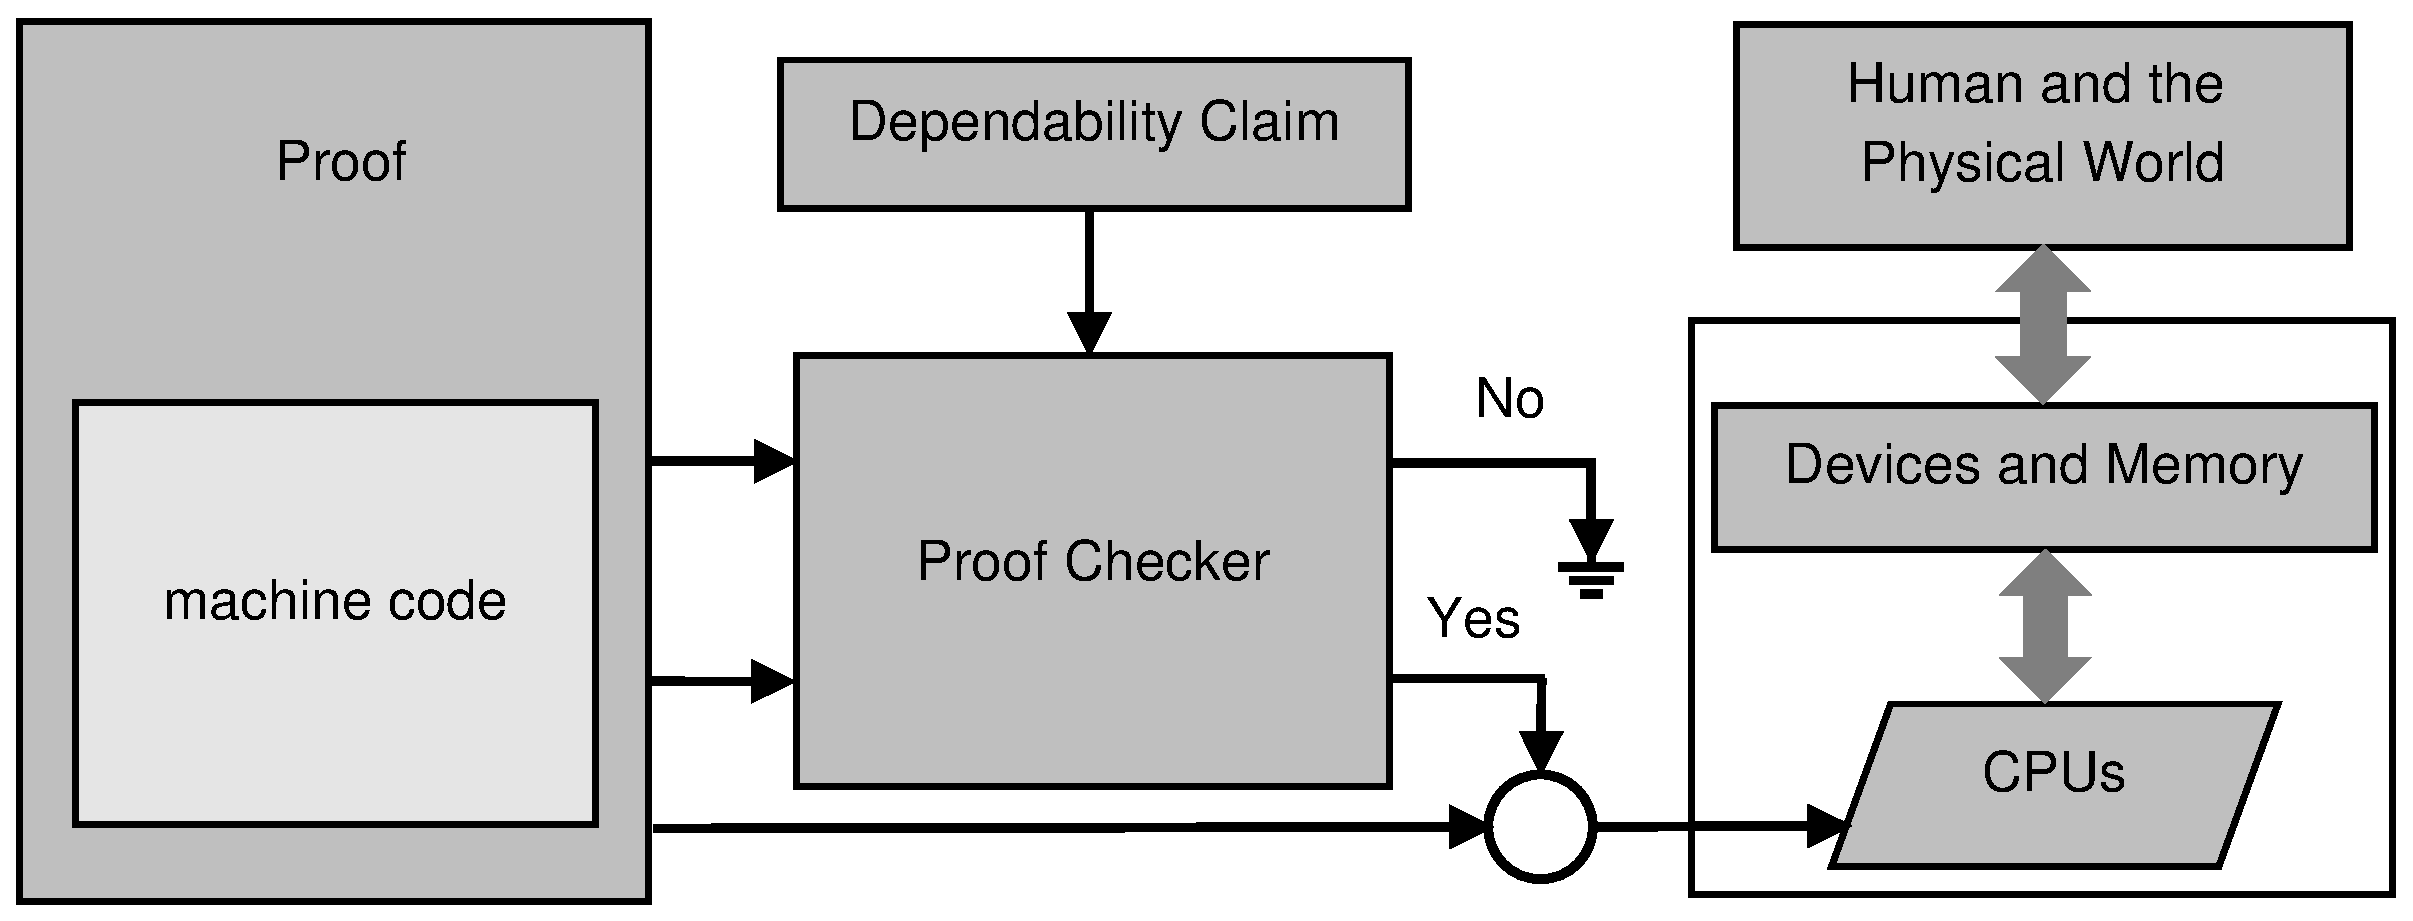
\includegraphics[height=1.5in ,width=3.4in]{framework.eps}
	\caption{Components of a typical certified framework (copied from \cite{shao})}
	\end{figure}

If the proof of a given certified software can be validated by the proof checker, then the execution of this software can be guaranteed to satisfy the dependability claim. On the other hand, considering that the proof checker itself is a computer program which could be bug-prone, the designers use simple logic with a small number of inference rules to write it, and verify it by hand, then make it the proof checker. By doing this the trustworthiness of the proof checker can be assured absolutely. 

For certified software itself, writing formal proofs and specifications and checking the validity of them by computer automatically is a core technique. According to Curry-Howard correspondence \cite{haskell}, in programming language theory and proof theory, types corresponds to propositions, programs corresponds to proofs and computation corresponds to simplification. If we prove the codes, the correctness will be ensured absolutely. Currently, this work is finished using the proof assistant \cite{coq}, which provides a rich higher-order logic with powerful inductive definitions. By using Coq, the framework could support explicit machine-checkable proof objects, and simplify the validation process by proof checker.


% An example of a floating figure using the graphicx package.
% Note that \label must occur AFTER (or within) \caption.
% For figures, \caption should occur after the \includegraphics.
% Note that IEEEtran v1.7 and later has special internal code that
% is designed to preserve the operation of \label within \caption
% even when the captionsoff option is in effect. However, because
% of issues like this, it may be the safest practice to put all your
% \label just after \caption rather than within \caption{}.
%
% Reminder: the "draftcls" or "draftclsnofoot", not "draft", class
% option should be used if it is desired that the figures are to be
% displayed while in draft mode.
%
%\begin{figure}[!t]
%\centering
%\includegraphics[width=2.5in]{myfigure}
% where an .eps filename suffix will be assumed under latex, 
% and a .pdf suffix will be assumed for pdflatex; or what has been declared
% via \DeclareGraphicsExtensions.
%\caption{Simulation Results}
%\label{fig_sim}
%\end{figure}

% Note that IEEE typically puts floats only at the top, even when this
% results in a large percentage of a column being occupied by floats.


% An example of a double column floating figure using two subfigures.
% (The subfig.sty package must be loaded for this to work.)
% The subfigure \label commands are set within each subfloat command, the
% \label for the overall figure must come after \caption.
% \hfil must be used as a separator to get equal spacing.
% The subfigure.sty package works much the same way, except \subfigure is
% used instead of \subfloat.
%
%\begin{figure*}[!t]
%\centerline{\subfloat[Case I]\includegraphics[width=2.5in]{subfigcase1}%
%\label{fig_first_case}}
%\hfil
%\subfloat[Case II]{\includegraphics[width=2.5in]{subfigcase2}%
%\label{fig_second_case}}}
%\caption{Simulation results}
%\label{fig_sim}
%\end{figure*}
%
% Note that often IEEE papers with subfigures do not employ subfigure
% captions (using the optional argument to \subfloat), but instead will
% reference/describe all of them (a), (b), etc., within the main caption.


% An example of a floating table. Note that, for IEEE style tables, the 
% \caption command should come BEFORE the table. Table text will default to
% \footnotesize as IEEE normally uses this smaller font for tables.
% The \label must come after \caption as always.
%
%\begin{table}[!t]
%% increase table row spacing, adjust to taste
%\renewcommand{\arraystretch}{1.3}
% if using array.sty, it might be a good idea to tweak the value of
% \extrarowheight as needed to properly center the text within the cells
%\caption{An Example of a Table}
%\label{table_example}
%\centering
%% Some packages, such as MDW tools, offer better commands for making tables
%% than the plain LaTeX2e tabular which is used here.
%\begin{tabular}{|c||c|}
%\hline
%One & Two\\
%\hline
%Three & Four\\
%\hline
%\end{tabular}
%\end{table}


% Note that IEEE does not put floats in the very first column - or typically
% anywhere on the first page for that matter. Also, in-text middle ("here")
% positioning is not used. Most IEEE journals/conferences use top floats
% exclusively. Note that, LaTeX2e, unlike IEEE journals/conferences, places
% footnotes above bottom floats. This can be corrected via the \fnbelowfloat
% command of the stfloats package.


\section{A simple Verification Example}

The most challenging part of certified software framework is how to write formal proof for a section of code using proof assistant. Simply speaking, what we need to do on verification must satisfy two properties. On one hand, the code should be free of probable threats, such as dead loop, arithmetic overflow and out-of-bounds array access; on the other hand, the code must meet the given functional requirements. Both the two properties can be written as annotations, which can be inserted directly into the source code like C code comments. A simple real example is shown in Figure 2.

%\begin{lstlisting}[title={Figure 2. Sterbenz----a simple C source code sample}, label=Csource]



%\noindent \texttt{/*}\\ 
%\texttt{@ requires y/2 <= x <= 2*y}\\
 %\texttt{ \hspace{2cm} @ ensures  \ result == x-y}\\
 % \texttt{@*/}\\

%\texttt{float Sterbenz(float x,float y)\{}  \\
%\texttt{ return x-y;}\\
%\texttt{\}}\\

%\begin{lstlisting}
\begin{figure}[H]
\begin{lstlisting}[label=Csource]

/*@ requires y/2 <= x <= 2*y
  @ ensures  \ result == x-y
  @*/

float Sterbenz(float x,float y){
  return x-y;
}
\end{lstlisting}    
\caption{Sterbenz----a simple C source code sample}
\end{figure}


The simple single precision C function in Figure 2 formally states the well-known Sterbenz theorem \cite{sterbenz}: if \emph{x} and \emph{y} are floating point numbers not too far away ($y/2 \le x \le 2y$), then $x-y$ is computed exactly. In this example, the preconditions and post-conditions of this function are inserted as comments of shape /*@...*/. The keyword \texttt{requires} introduces all preconditions, before the function is carried out, these required properties must be satisfied first; the keyword \texttt{ensures} introduces all post-conditions, when the function returns, these properties must be assured; the keyword \texttt{\char92 result} describes the return value.

When run on the source code with such annotations, the formal verification tool at the C source code level will produce a single verification condition in Figure 3 automatically.

\begin{figure}[H]
\begin{lstlisting}[label=intermediate]

$\forall x$ : single. $\forall y$ : single.

s_to_$r(y)/2 \le $s_to_r$(x) \le 2 \times $s_to_r$(y) \Rightarrow$

    s_to_r(sub_single(nearest_even, $x$, $y$)) $=$ 

    s_to_r($x$)$-$s_to_r($y$)

\end{lstlisting}    
\caption{Intermediate verification for Sterbenz function}
\end{figure}


%$\forall x : \texttt{single}.  \forall y : \texttt{single}.$\\
%$\texttt{s\_to\_r}(y)/2 \le  \texttt{s\_to\_r}(x) \le 2 \times  \texttt{s\_to\_r}(y) \Rightarrow$

The meanings of related keywords in the above intermediate code are as follows:

\texttt{single}: projection to data type, here means single precision float

\texttt{s\_to\_r}: projection to access the floating-number part;

\texttt{sub\_single}: projection to subtraction on the type \texttt{single};

\texttt{nearest\_even}: projection to the rounding mode, by default, rounding to nearest, ties to even.

Next, this verification condition can be transformed using Coq tactics, here is the core part of corresponding proof by Sylvie Boldo \cite{Boldo}:

\begin{figure}[H]
\begin{lstlisting}[label=Coq]
...
Proof.
  intros x; intros; 
  apply bounded_real_no_overflow_single.
  cut (0 <= single_value y)%R; try intros.
  cut (0 <= single_value x)%R; try intros.
  case (Rle_or_lt(single_value x)(single_value y)); 
  intros. rewrite Rabs_left1; ring_simplify.
  apply Rle_trans with(-0+single_value y)%R;
  auto with real. ring_simplify; 
  rewrite <- (Rabs_right (single_value y));
  [apply single_le_strict|auto with real.]
  apply Rplus_le_reg_l with(single_value y); 
  now ring_simplify. rewrite Rabs_right; 
  ring_simplify.
  apply Rle_trans with(single_value x-0)%R.
  apply Rplus_le_compat_l; auto with real.
  ring_simplify; 
  rewrite <- (Rabs_right(single_value x));
  [apply single_le_strict|auto with real].
  apply Rle_ge; 
  apply Rplus_le_reg_l with(single_value y); 
  ring_simplify; auto with real.
  apply Rle_trans with(single_value y/2)%R;
  [idtac|apply HW_1].unfold Rdiv; 
  apply Rmult_le_pos; auto with real.
  apply Rmult_le_reg_l with 3%R;
  [apply Rlt_le_trans with 2%R;auto with real|idtac].
  apply Rplus_le_reg_l with(single_value y); 
  apply Rmult_le_reg_l with(/2)%R; auto with real.
  replace (/2*(single_value y + 3*0))%R 
  with (single_value y/2)%R by(unfold Rdiv; ring).
  apply Rle_trans with(single_value x);
  [eapply HW_1|idtac].
  apply Rle_trans with(2*single_value y)%R;
  [eapply HW_1|right;field].
Save.
\end{lstlisting}    
\caption{A section of proof in Coq}
\end{figure}

The keywords such as \texttt{intros, apply } and \texttt{rewrite} stand for Coq tactics, which are used for constructing complex proofs semi-automatically. The keywords like \texttt{bounded\_real\_no\_overflow\_single} and \texttt{Rplus\_le\_reg\_l} are lemmas defined by provers. This section of Coq proof code seems quite long, and the whole proof online is even much longer \cite{proof}. However, most of code will be generated by Coq assistant automatically, and the real proof process is not very difficult. The proof written by Coq will be checked for validation by proof checker in next step.


\section{A realistic example---certified compiler}

In recent years, the verification technique has been used in various types of practical software projects, such as assembly programming languages, compilers and proof assistants. Necula's and Lee's work on proof-carring code (PCC) is the immediate precursor to the large body of more recent work on certified software \cite{Necula}. Yu et al. in \cite{CAP} propose a low-level language, Certified Assembly Programming, for building certified programs and present a certified library for dynamic storage allocation. McCreight et al. in \cite{garbage} develop a general framework for certifying a range of garbage collectors. Feng et al. in \cite{thread} certify the partial correctness of a preemptive thread library extracted from our simplified OS kernel.  



Leroy verifies a realistic compiler for the first time \cite{compiler}. Compilers are software that perform complicated semantic and symbolic transformations, and also bug-prone low-level programs. That means if the compiler itself is not trustworthy, it may generate incorrect executable machine code probably, no matter how correct the source program is. Figure 2 shows a simple common bug in the GCC compiler \cite{gccbug}. Here a bug appears because C99 allows intermediate results to be computed with excess precision, but requires them to be rounded at assignments.

\begin{figure}[H]
\begin{lstlisting}[label=gccbug]
#include <stdio.h>

void test(double x, double y)
{
  const double y2 = x + 1.0; //not rounded to 64 bits
  if (y != y2) printf("error");
}

void main()
{
  const double x = .012;
  const double y = x + 1.0; //rounded to 64 bits

  test(x, y);
}
\end{lstlisting}
\caption{A bug caused by GCC}
\end{figure}

For non-critical software such as web game applications, compiler-caused bugs are often negligible because the developers rarely run into them. But when they have to tackle this, debugging will be very difficult. For critical software like military and financial software systems, this insidious threat should be seriously considered. The traditional testing methods are no longer effective here, and need to be replaced by using formal methods such as program verification. Otherwise, the test plan will be very complicated and expensive. However, even the guarantees obtained by formal verification in source code level may not lead to 100\% trustworthy executable code because of the possible miscompilation, which means the compiler creates incorrect output from correct input.

A solution to this tough problem is using certified compiler. The core idea of certified compiler is using formal proof to the compiler itself to prove that the compiler preserves the semantics of the source code. If the compilation succeeds, the generated machine code should behave as prescribed by the semantics of the source code. Leroy et al. develop and verify a realistic compiler--CompCert, which is useable for critical embedded software. The source language of CompCert is named Clight. Clight is a very large subset of C programming language. It supports most of data types in C, such as \texttt{struct}, arrays and pointers; it also supports all C-style expressions (including pointer arithmetic), control (loops, \texttt{break}, \texttt{continue} and \texttt{if/then}), functions (including recursive functions and function pointers) and volatile accesses. The target code can be PowerPC, ARM or x86 assembly language code \cite{CompCert}.


	\begin{figure}[H]
	\centering
	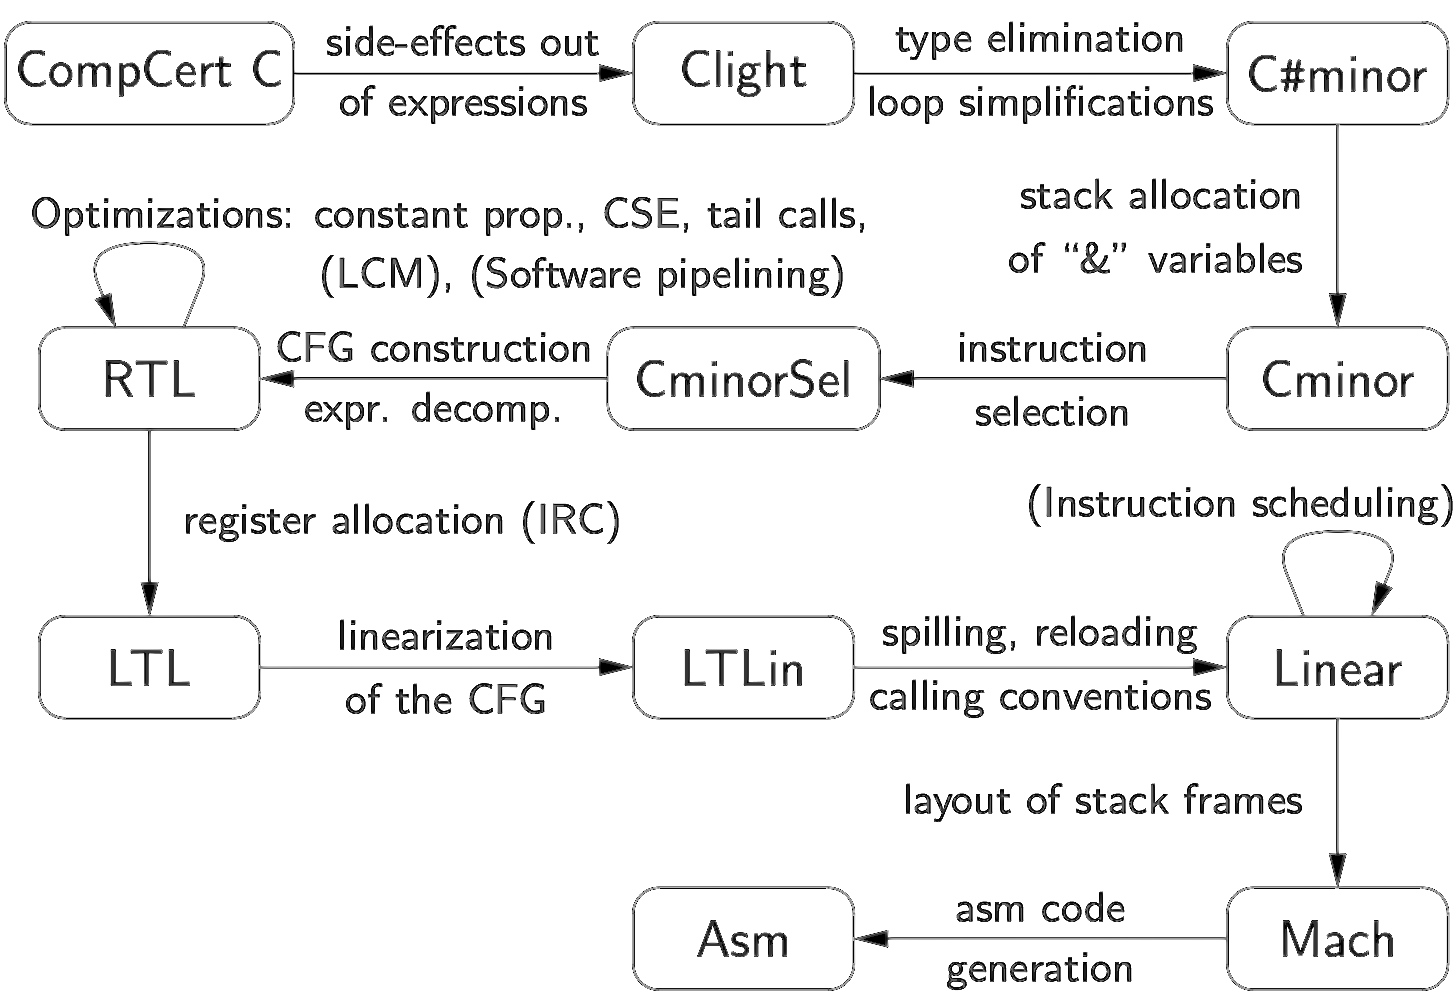
\includegraphics[height=2.4in ,width=3.4in]{compiler.png}
	\caption{The formally verified part of the compiler (copied from \cite{compiler})}
	\end{figure}

The whole compliation process for CompCert is shown in figure 6. All the compilation steps in CompCert are standard steps used in all compilers, but each step is proved correct using Coq assistant, and the correctness proofs are the special part which is different from other compilers.

In the beginning, the compiler translates source Clight code into C\#minor and Cminor intermediate code, during these two steps, all type-dependent behaviors will be removed. Then, the compiler selects suitable arithmetic instructions, such as add-immediate and not-and, to rewrite Cminor code to CminorSel, which is a processor-dependent variant of Cminor. Additional operators and addressing modes will be introduced in this step. Next, the CminorSel will be translated to register transfer language (RTL). The developers do optimizations in this step, because in RTL control can be represented as a control-flow graph and each node corresponds to a machine-level instruction. When optimizations are finished, the compiler will allocate registers to generate a language called location transfer language (LTL). In this subprocess, the compiler use registers or stack locations to replace previous temporaries.

Now, the compiler will carry out code linearization to linearize the control-flow graph, and replace LTL using lists of instructions with explicit labels and branches to these labels in the style of assembly code. The branches include both conditional and unconditional ones. The output target language is LTLin. Usually, two or three transitions in LTLin correspond to one intra-function transition in the original LTL code. The next step finishes the register allocation process, using "spilling" and "reloading" methods \cite{compiler}. Instructions like \texttt{move} are inserted around function calls in this step, too. After this, the compiler will allocate space for stack and turn the accesses to stack into memory instructions \texttt{load} and \texttt{store}. The output is called Mach, which is very close to the final assembly language in semantics. In the final compilation step, the real assembly language code will be generated.

The original semantics are proven to be preserved by Coq in each step. The author's experiments show that the final executable machine code generated by CompCert outperforms the one generated by GCC without optimizations, and even competitive with GCC at optimization level 1 (\texttt{gcc -O1}) and 2 (\texttt{gcc -O2}). In 2011, Yang et al. build CSmith, which is tool for finding bugs in C compilers, and use it to perform random testing among C compilers like GCC and Clang \cite{CSmith}. Until now they have found 79 bugs in GCC, however, they found no bug in CompCert.

\section{Testing or proof}

As can be seen from above, using formal proof to improve the software security is a very complicated and effort-consuming process. A probable question is whether this technique should be adopted by industry. Because small software companies may not afford such a cost financially. However, on the other hand, the technique people are using in reality nowadays, software testing, is labor-intensive, too. The core question is for those non-critical software development, to improve the security, which one is more cost-effective?

Steve King et al. answer this question, and show both the advantages and feasibility of industrial-scale proof on commercial software projects, and show that using proof is more cost-effective than traditional testing method in \cite{testing}. They use formal proof and testing at the same time to find the faults in a real commercial software called SHOLIS project, which consists of 133,000 lines of Ada code. The authors compare the proof with various types of testing (e.g. unit testing, integration testing and system validation testing), and make analysis based on engineering judgment instead of theoretical computer science. The final result shows that the overall performance of industrial-scale proof is much better than the authors expect originally. Z proof, which is a formal proof technique they use in the paper, even outperforms the most efficient testing method on finding faults.

\section{Summary and future work}

Certified software is a fast developing technique. In this paper we simply review some recent classical papers on this topic. Among all the components in a certified software framework, how to write formal proof for source code is the most confusing part for beginners. We use simplest example to illustrate the basic working process of formal verification, using both a simple C program example and a practical certified complier example. We also take the SHOLIS project for example to illustrate that using verification for quality assurance is more cost-effective than testing.

After the CompCert experiment, the goal of proving the correctness of a realistic compiler appears feasible. Considering the fact that the methodologies, techniques and tools used are far from perfect, Leroy's work opens up many directions for our own work in future. For example, we can extend Leroy's work to handle a larger subset of C, deploy and prove the correctness of more optimizations. Further, we can set up a model to prove the correctness of an assembler and linker, at least constitutes a first step towards these more complex goals, using formal methods and verification tools. 

Considering the complexity of CompCert, adding new features (e.g. \texttt{goto} sentence) or optimization to CompCert may cause existing programs to fail. Because new bugs might be introduced into the proved compiler, and we have to prove the whole compiler again to check its trustworthiness. So, in the near future, we will focus on performing translation validation \cite{translation} with formal proof methods, which requires only the verification of the compiler output, not the whole compiler implementation itself. 

The principal challenge on this topic is expressing algorithms as provable Coq functions. We will use inductive predicates with inference rules to specify an algorithm in our framework, and by doing this we can make the most of previous work like \cite{validator}. Our semantic functions will be constructed as follows: First of all, we state the correctness of a semantic function \emph{f} as a property relating the input and its output. At the same time, we state specification \emph{Q} for the function \emph{f} as its preconditions and postconditions. Secondly, we create a function called \emph{certifying function} to return two things: the justified result of the output of \emph{f} (denoted as \emph{R}), and a proof that shows \emph{R} satisfies \emph{Q}. Next, when the function \emph{f} calls other functions, the related certifying functions and proofs will be given accordingly. Finally, we can combine all subproofs using appropriate logic rules  to demonstrate the whole translation is proven to be validated.

This method will be very hard for long and complex functions probably, but we will keep trying. We hope to establish a more effective translation validator framework for CompCert with Coq proof assistant, which is helpful to the researchers in this area. 



% conference papers do not normally have an appendix


% use section* for acknowledgement
\section*{Acknowledgment}

We would like to thank Prof. Daniel Lopresti, Prof. Gang Tan, and Dr. Maryann DiEdwardo for their helpful and valuable feedback on earlier versions of the paper.


% trigger a \newpage just before the given reference
% number - used to balance the columns on the last page
% adjust value as needed - may need to be readjusted if
% the document is modified later
%\IEEEtriggeratref{8}
% The "triggered" command can be changed if desired:
%\IEEEtriggercmd{\enlargethispage{-5in}}

% references section

% can use a bibliography generated by BibTeX as a .bbl file
% BibTeX documentation can be easily obtained at:
% http://www.ctan.org/tex-archive/biblio/bibtex/contrib/doc/
% The IEEEtran BibTeX style support page is at:
% http://www.michaelshell.org/tex/ieeetran/bibtex/
%\bibliographystyle{IEEEtran}
% argument is your BibTeX string definitions and bibliography database(s)
%\bibliography{IEEEabrv,../bib/paper}
%
% <OR> manually copy in the resultant .bbl file
% set second argument of \begin to the number of references
% (used to reserve space for the reference number labels box)
\begin{thebibliography}{1}

  
  \bibitem{shao}Z. Shao, Certified software. \emph{Communications of the ACM}, 53(12):56-66, 2010.

  \bibitem{compiler} X. Leroy. Formal verification of a realistic compiler. \emph{Communications of the ACM}, 52(7):107-115, 2009.

  \bibitem{haskell} C. Haskell, Functionality in Combinatory Logic. \emph{In Proceedings of the National Academy of Sciences 20}, pp. 584-590, 1934.

  \bibitem{coq} G. Huet, C. Paulin-Mohring, et al. \emph{The Coq proof assistant reference manual}. The Coq release v6.3.1, May 2000.
    
  \bibitem{sterbenz} P. H. Sterbenz. \emph{Floating point computation}. Prentice Hall, 1974.
    
  \bibitem{float}  S. Boldo, J.C. Filli\^atre. Formal verification of floating-point programs. \emph{In IEEE Symposium on Computer Arithmetic}, pp. 187-194, 2007.
    
    \bibitem{CompCert} The CompCert verified compiler. \url{http://compcert.inria.fr/doc/}
    
   \bibitem{Boldo} Sylvie Boldo's homepage. \url{https://www.lri.fr/~sboldo/research.html}
  
   \bibitem{proof} Full Coq proof of Sterbenz's theorem. \url{https://www.lri.fr/~sboldo/progs/Sterbenz\_why.v}
   
   \bibitem{gccbug} Bug 323--optimized code gives strange floating point results. \url{http://gcc.gnu.org/bugzilla/show\_bug.cgi?id=323}
   
    \bibitem{testing} S. King, J. Hammond, R. Chapman, and A. Pryor. ``Is Proof More Cost-Effective Than Testing?" \emph{IEEE Transanctions on Software Engineering}, 26(8):675-686, 2000.

  \bibitem{Necula} G. Necula, P. Lee. Safe kernel extensions without run-time checking. \emph{In Proceedings of the 2nd USENIX Symposium on Operating System Design and Implementation}, pp. 229-243, 1996.

  \bibitem{CAP} D. Yu, N. A. Hamid, and Z. Shao. Building certified libraries for PCC: Dynamic storage allocation. \emph{In Proceedings of the 2003 European Symposium on Programming}, vol. 2618 of LNCS, pp. 363-379, 2003.

  \bibitem{garbage} A. McCreight, Z. Shao, C. Lin, and L. Li. A general framework for certifying garbage collectors and their mutators. \emph{In Proceedings of  2007 ACM Conference on Programming Language Design and Implementation}, pp. 468-479, 2007.

  \bibitem{thread} X. Feng, Z. Shao, Y. Dong, and Y. Guo. Certifying low-level programs with hardware interrupts and preemptive threads. \emph{In Proceedings of 2008 ACM Conference on Programming Language Design and Implementation}, pp. 170-182, 2008.

  \bibitem{CSmith} X. Yang, Y. Chen, E. Eide, and J. Regehr. Finding and understanding bugs in C compilers. \emph{In 32nd ACM SIGPLAN Conference on Programming Language Design and Implementation}, pp. 283-294, 2011.
  
  \bibitem{translation} A. Pnueli, M. Siegel, and E. Singerman, Translation validation. \emph{In Tools and Algorithms for Construction and Analysis of Systems}, vol. 1384 of LNCS, pp. 151-166, 1998.
  
  \bibitem{validator} J. B. Tristan, X. Leroy. Formal verification of translation validators: a case study on instruction scheduling optimizations. \emph{In 35th Symposium Principles of Programming Languages}, pp. 17-27, 2008.
  


\end{thebibliography}




% that's all folks
\end{document}


